\documentclass[a4paper, 11pt, twoside]{article}

\usepackage[english]{babel}
\usepackage{titlesec}

\usepackage{afterpage}
\usepackage{makeidx}
\usepackage[hyphenbreaks]{breakurl}

\usepackage{caption}
\captionsetup[figure]{font=small}
\usepackage{subcaption}
\newcommand{\source}[1]{\caption*{Source: {#1}} }

\usepackage{tocloft}
\renewcommand{\cftsecleader}{\cftdotfill{\cftdotsep}}
\renewcommand{\figurename}{Figure}

\usepackage{cancel}

\usepackage[utf8]{inputenc}

\usepackage{mathtools}

\usepackage{amsmath}

\usepackage{graphicx}
\usepackage{multicol,lipsum}

\usepackage{listings}
\usepackage{indentfirst}

\usepackage[T1]{fontenc}

\usepackage{comment}
\usepackage{float}

\usepackage{pdfpages} % Package para pdf segundo o Stack Overflow

\usepackage{color, colortbl}

\usepackage{sectsty}

\usepackage[a4paper, total={6in, 9in}]{geometry}
\usepackage{blindtext}
\usepackage{lastpage}

\geometry{
  inner= 2.5 cm, 
  outer= 2.5 cm,
  top= 2.5 cm,       % Margem superior
  bottom= 2.5 cm     % Margem inferior
}

\usepackage{fancyhdr}

\pagestyle{fancy}
\fancyhf{} % limpa tudo

% Usa slots para páginas pares e ímpares (funciona em one/two-side)
\fancyhead[LE,LO]{Network Virtualization in Data Centers}
\fancyhead[RE,RO]{Group 5}

\renewcommand{\headrulewidth}{0.4pt}
\fancyfoot[C]{\thepage}
\setlength{\headheight}{15pt}

% Torna o estilo "plain" (usado por TOC/LOF) igual ao acima
\fancypagestyle{plain}{
  \fancyhf{}
  \fancyhead[LE,LO]{Network Virtualization in Data Centers}
  \fancyhead[RE,RO]{Group 5}
  \renewcommand{\headrulewidth}{0.4pt}
  \fancyfoot[C]{\thepage}
}

\usepackage{listings}
\usepackage{graphicx}
\usepackage{caption}
\usepackage{wrapfig}

\usepackage{hyperref}
\usepackage{cleveref}

\usepackage{tocloft}

\makeatletter
\renewcommand*\l@figure{\@dottedtocline{1}{0em}{0em}}
\makeatother

\setlength{\cftafterloftitleskip}{40pt}

\makeatletter
\renewcommand{\l@figure}[2]{%
  \begingroup
    \renewcommand{\numberline}[1]{Figure~##1:\enspace}%
    \@dottedtocline{1}{1em}{1em}{#1}{#2}%
  \endgroup
}
\makeatother

\usepackage{lipsum}
\usepackage{hyperref}

\usepackage{titlesec}
\usepackage{tocloft}

\usepackage{hyperref}
\let\oldunderbar\underbar
\renewcommand{\underbar}[1]{\oldunderbar{#1}}


\renewcommand{\cfttabpresnum}{}
\renewcommand{\cfttabaftersnum}{}
\setlength{\cftfignumwidth}{0pt} 
\setlength{\cfttabnumwidth}{0pt} 

\usepackage[backend=biber,style=ieee]{biblatex}
\addbibresource{refs.bib}

\usepackage[acronym]{glossaries}
\usepackage{acronym}
\makeglossaries
% ------------------------ Capa ------------------------ 
\begin{document}

\begin{titlepage} % Criar página de título personalizada

    \begin{center} % centrar
        

        \vspace{50pt}
    
        \begin{figure}[h] % \begin{figure}[place]
            \centering
            
\includegraphics[scale = 1]{Figures/feup.png}
        \end{figure}
    
        \vspace{50pt} % espaço vertical de 50pt
    
        \LARGE{\textbf{Network Virtualization in Data Centers}} \par 

        \vspace{50pt}

        \normalsize{ 
        \begin{tabular}{ccc}
            \textbf{André Silva} & \textbf{Leonor Guedes} & \textbf{Rafael Parody} \\
            up202107419 & up202107691 & up202502656 \\
        \end{tabular}
        }

        \mbox{}
        \vfill
        
        \normalsize{ 
        Carried out within the scope of the\\
        “Telecommunications Networks” course\\
        of the Master's in Electrical and Computer Engineering\\
        }
        \vspace{50pt}
        \normalsize{7 of November of 2025}


        
    \end{center}

\end{titlepage}

% ------------------------ Fim Capa ------------------------
\pagenumbering{roman}
\setcounter{page}{2}

\section*{Abstract}

\paragraph{}

\pagebreak

% ----------- índice -----------
\tableofcontents


\newpage

% ----------- Lista de Figuras -----------

\listoffigures

\newpage
% ----------- Abreviaturas -----------
\section*{List of Abbreviations}
\paragraph{}
\begin{acronym}[NVGRE] % 
  \acro{DC}{Data Center}
  \acro{ECMP}{Equal-Cost Multi-Path}
  \acro{eBGP}{External Border Gateway Protocol}
  \acro{Geneve}{Generic Network Virtualization Encapsulation}
  \acro{GRE}{Generic Routing Encapsulation}
  \acro{GTEP}{Geneve Tunnel Endpoint}
  \acro{HNV}{Hyper-V Network Virtualization}
  \acro{IP}{Internet Protocol}
  \acro{LAN}{Local Area Network}
  \acro{MTU}{Maximum Transmission Unit}
  \acro{NVGRE}{Network Virtualization using Generic Routing Encapsulation}
  \acro{OAM}{Operations, Administration and Maintenance}
  \acro{OSPF}{Open Shortest Path First}
  \acro{OSI}{Open Systems Interconnection}
  \acro{OVS}{Open vSwitch}
  \acro{TLV}{Type-Length-Value}
  \acro{UDP}{User Datagram Protocol}
  \acro{VDC}{Virtualized Data Center}
  \acro{VLAN}{Virtual Local Area Network}
  \acro{VNI}{VXLAN Network Identifier}
  \acro{VN}{Virtual Network}
  \acro{VTEP}{VXLAN Tunnel Endpoint}
  \acro{VXLAN}{Virtual Extensible LAN}
  \acro{VM}{Virtual Machine}
\end{acronym}


\newpage

% ----------- 
\pagenumbering{arabic}

\section{Introduction}
\paragraph{}
Nowadays, modern organizations rely on rapidly expanding data centers capable of supporting increasingly demanding workloads. Consequently, the data center network must ensure the efficient isolation, mobility, and scalability of these workloads without introducing complexity into the physical infrastructure. This is achieved by operating primarily at the logical layer, allowing changes in network configuration and segmentation without modifying the physical core.

Traditional VLAN-based segmentation techniques are limited in scale and flexibility, offering only 4096 identifiers, which is insufficient for the dynamic and multi-tenant nature of modern data centers. To overcome these constraints, network overlays enable the creation of virtual networks that operate on top of an existing physical underlay. Through encapsulation mechanisms, overlays transport Layer 2 traffic over a Layer 3 infrastructure, providing logical isolation and improved workload mobility across the data center fabric.

This report provides an overview of network virtualization in data centers, examining its core components, underlying technologies, and operational principles. In addition, it is considered the control and orchestration mechanisms that enable automation and scalability, as well as the integration between physical and virtual infrastructures and the security challenges arising from this paradigm.

The structure of this report is organized to provide a logical progression from fundamental concepts to advanced topics. In section 2 is introduced the main principles of network virtualization, followed by Section 3, which examines the most relevant overlay technologies. Section 4 describes the control and orchestration mechanisms that enable automation and scalability, while Section 5 focuses on the integration between physical and virtual layers. Finally, section 6 discusses security and compliance considerations.
\section{Data Center}

This section aims to provides an overview of the main architectural principles that underpin modern data centers. It is explored the separation between the physical and virtual network layers as well as how these components interact to deliver scalability and reliability in large-scale environments.

\subsection{Overview}
\paragraph{}
Data centers are physical facilities designed to house information systems and telecommunications equipment, as well as to process and distribute large volumes of data securely and efficiently. They integrate cooling systems, redundant power supplies and both physical and logical controls to ensure the continuous and reliable operation of organizations.\par

A data centers is generally divided into five main blocks. The first is the physical infrastructure, which encompasses racks, structured cabling, cooling systems, and fire detection and suppression systems. The second is data processing and storage, including both physical and virtualized servers, storage arrays, and associated systems. The third component is the network infrastructure, the key to operations, which interconnects the data center with external environments, such as cloud services or remote sites, comprising routers, firewalls and switches. The fourth component is the management system, responsible for event logging, continuous monitoring, and maintaining environmental stability. Finally, the fifth component corresponds to the security mechanisms, which protects data through physical and logical controls, including network segmentation (VLAN, VNI), access policies and encryption in transit and at rest. \par

The predominant network architecture in today's data centers is the leaf-spine IP mesh, which operates at Layer 3 of the OSI model. The underlay typically employs a high Maximum Transmission Unit (MTU) to support encapsulation overhead and relies on stable routing protocols, such as eBGP and OSPF. The overlay network is built atop this physical fabric, providing logical segmentation and workload mobility without IP addresses modification. Technologies such as VXLAN, NVGRE and Geneve are central to this virtualized architecture and will be examined in greater depth in subsequent sections.\par

\subsection{Data Center Network Architecture}
The foundation of modern data centers lies in the separation between the underlay, which represents the physical network infrastructure, and the overlay, which comprises the virtual networks. 
\newpage
\begin{wrapfigure}{r}{0.48\textwidth}
    \centering
    \vspace{-5pt}
    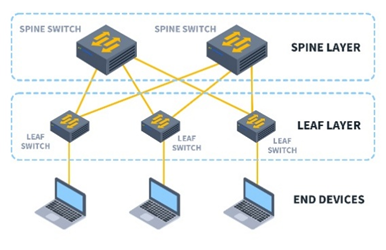
\includegraphics[width=0.9\linewidth]{Figures/LeafSpine.png}
    \caption{Leaf-spine structure. \cite{leafspine}}
    \label{leafSpine}
    \vspace{-10pt}
\end{wrapfigure}

The underlay corresponds to the physical IP fabric of the network, typically organized in a Layer 3 leaf-spine topology. This topology, as illustrated in Figure \ref{leafSpine}, consists of two layers: the spine, formed by high-speed switches that constitute the network backbone; and the leaf, consisting of access switches that connect servers, storage devices and other endpoints. The primary objective of the underlay is to transport packets quickly and efficiently. For this reason, a high MTU, usually around 9000 bytes, is used to to accommodate encapsulation overhead and minimize fragmentation. 

The overlay is built on top of this fabric and consists of a set of virtual networks that encapsulate each user's traffic, providing logical isolation and mobility, without changing IP addresses. In practice, encapsulation mechanisms such as VXLAN, NVGRE or Geneve are employed. Each virtual network is identified by a unique segment ID, enabling scalable segmentation within large infrastructures. The central component of the overlay is the VXLAN Tunnel Endpoint (VTEP), typically residing on a leaf switch, responsible for encapsulating and decapsulating traffic between the overlay and the IP underlay. These virtual networks are often integrated with orchestration and automation platforms, which facilitate dynamic provisioning, policy enforcement and scalability. 

Correct MTU configuration within the underlay is critical, as an insufficient MTU will result in packet packet fragmentation and drops. Therefore, it is essential to maintain a adequately large MTUs and continuously monitor fragmentation and transmission metrics. The use of UDP-based encapsulation enhances multiple available paths through Equal-Cost Multi-Path (ECMP) routing, improving flow distribution, maximizing the inherent parallelism of the leaf-spine architecture and improving overall network efficiency. \par

\subsection{Data Centers Virtualization}

A Virtualized Data Center (VDC) is a data center where some or all the hardware components, such as servers, routers, switches and network links, are virtualized. Typically, a physical hardware is virtualized using software or firmware known as hypervisor, which divides the equipment into multiple isolated and independent  

\begin{wrapfigure}{r}{0.45\textwidth}
    \centering
    \vspace{-10pt}
    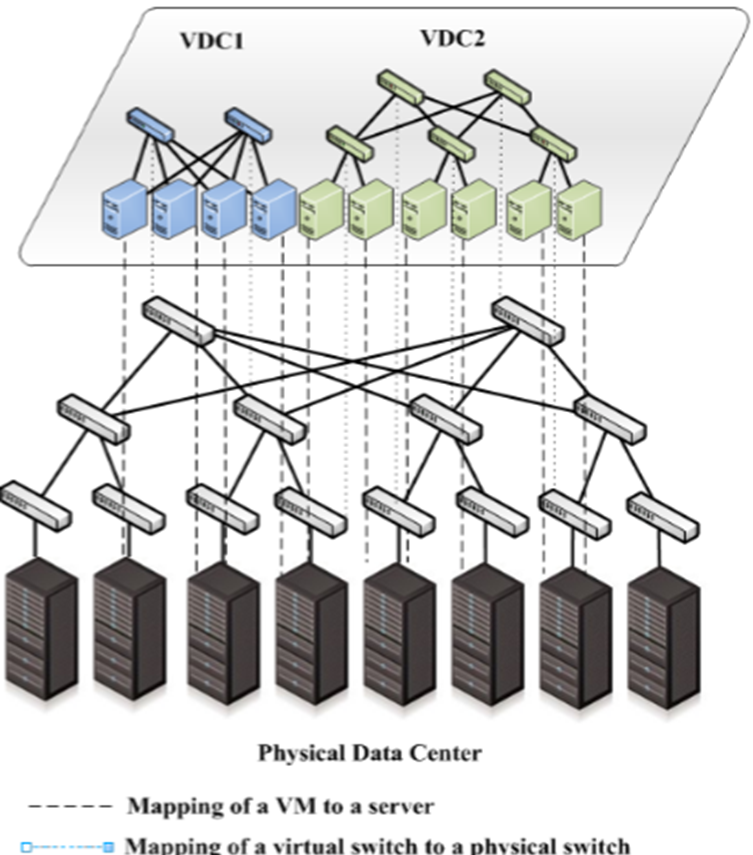
\includegraphics[width=0.8\linewidth]{Figures/virtualization.png}
    \caption{Virtualization of a Data Center. \cite{bari2013datacenter}}
    \label{virtualization}
    \vspace{-10pt}
\end{wrapfigure}

\noindent virtual instances. 

A VDC is defined as a collection of virtual resources, including VMs, virtual switches, and virtual routers, connected via virtual links and therefore constitutes a segment of a Virtual Data Center. While a Virtualized Data Center is a physical data center with deployed resource virtualization techniques, a Virtual Data Center is a logical instance of a Virtualized Data Center consisting of a subset of the physical data center resources. 

A Virtual Network (VN) is a set of virtual networking resources, such as virtual nodes (end-hosts, switches, routers) and virtual links and therefore, a VN is a part of a VDC. A network virtualization level is one of the layers of the network stack (application to physical) in which the virtualization is introduced. Figure \ref{virtualization}, shows how several VDCs can be deployed over a virtualized data center. 

\section{Overlay Network Technologies}
After defining the fundamental architecture of modern data centers, the following section examines the core technologies that enable network virtualization.

\subsection{Virtual Extensible LAN}
Traditional Virtual Local Area Networks (VLANs) have long been used to logically segment Layer 2 networks within a limited broadcast domain, identified by a 12-bit VLAN ID that supports up to 4096 tenants. In conventional Layer 2 switches, communication between servers connected to the same device is natively supported. When a server is migrated from one port of the Layer 2 switch to another port, its IP address can remain unchanged, satisfying the requirements for dynamic VM migration. However, as data centers evolved, VLANs began to show limitations, particularly in large-scale environments that require workload mobility and multi-tenant isolation. To overcome these constraints, the Virtual Extensible LAN (VXLAN) technology was introduced.

VXLAN is a network virtualization technology designed to extend Layer 2 connectivity across Layer 3 networks. It establishes a logical tunnel between network devices, through which it employs a MAC-in-UDP encapsulation mechanism for packet transport. In this model, original Ethernet frames generated by a Virtual Machine (VM) are encapsulated into UDP packets. These packets are then wrapped with IP and Ethernet headers of the physical network as outer headers, allowing them to be routed as standard IP traffic. This design removes the structural limitations of traditional Ethernet domains and enables greater scalability and isolation within modern data centers.
\newpage
\begin{figure} [H]
    \centering
    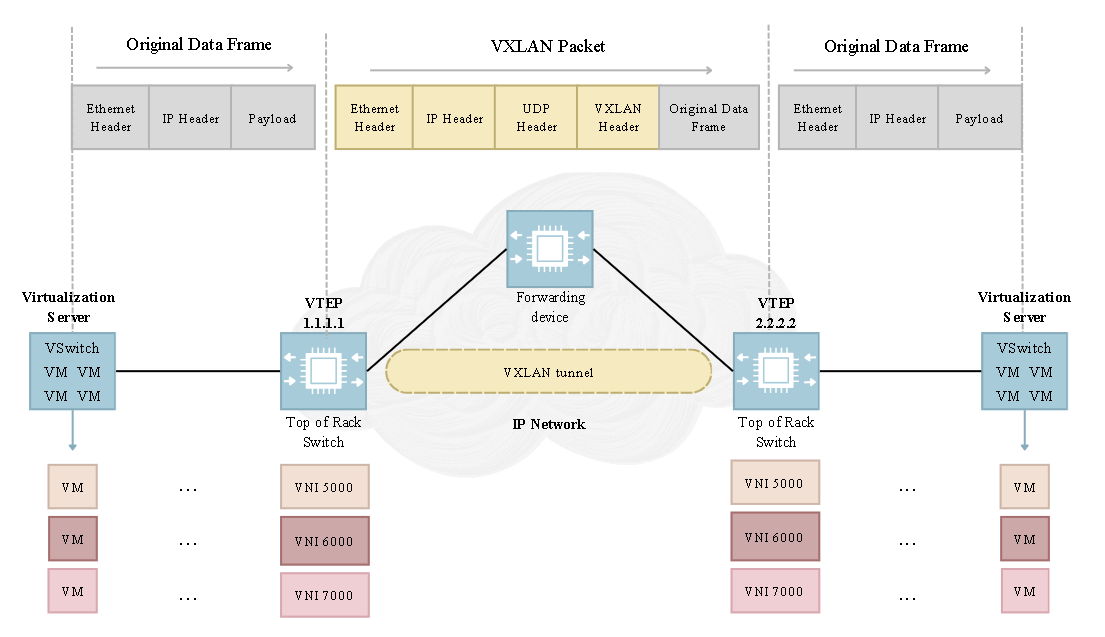
\includegraphics[width=0.9\linewidth]{Figures/VXLANmodel.png}
    \caption{VXLAN network model. \cite{ipwithease_vxlan}}
    \label{VXLANmodel}
\end{figure}

As shown in Figure \ref{VXLANmodel}, VXLAN extends Layer 2 communication over an IP underlay, creating a virtualized network that behaves as a single logical switch interconnecting all endpoints. Any two nodes can communicate transparently through VXLAN tunnels, regardless of the underlying physical topology. From the server's perspective, VXLAN virtualizes the entire infrastructure network into a large "Layer 2 virtual switch", interconnecting all servers as if they resided on the same Layer 2 segment. VXLAN therefore plays an important role in modern data centers as it leads to a significant increase in the number of tenants that the network can effectively isolate and manage. 

In terms of scalability, VXLAN uses a 24-bit VXLAN Network Identifier (VNI), allowing the identification of up to 16 million tenants, far higher than the supported by VLANs. Furthermore, in terms of migration flexibility, VXLAN establishes virtual tunnels between switches across the underlying IP network, effectively virtualizing the infrastructure into a large logical Layer 2 domain that supports large-scale dynamic VM migration.

\subsubsection{VXLAN Encapsulation Structure}

The VXLAN encapsulation process is illustrated in Figure \ref{VXLANpacket}, where the original Ethernet frame is encapsulated within UDP and IPv4 headers and transmitted over the underlay network.

\begin{figure} [H]
    \centering
    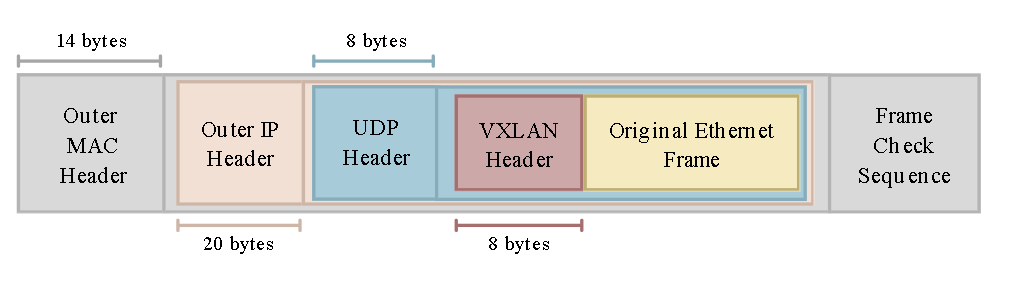
\includegraphics[width=0.65\linewidth]{Figures/VXLANpacket.png}
    \caption{VXLAN packet format. \cite{QSFPtekVXLAN}}
    \label{VXLANpacket}
\end{figure}

The VXLAN header, with a total length of 8 bytes, carries a 24-bit VNI, which uniquely identifies each virtual network or tenants within the VXLAN network. It also contains an 8-bit Flags field, typically set to 00001000, indicating the presence of a valid VNI, along with two reserved fields of 24 and 8 bits that are maintained for future use and protocol consistency.

The VXLAN header and the original Ethernet frame are transported as UDP data. Within the UDP header, the destination port number is fixed at 4789, while the source port number is dynamically calculated using a hash algorithm based on the original Ethernet frame. 

In the outer IP header, the source IP address corresponds to the VXLAN Tunnel Endpoint (VTEP) connected to the source VM, while the destination IP address identifies the VTEP connected to the destination VM. These addresses enable communication across the IP underlay network.

Finally, the outer MAC header, also known as the outer Ethernet header, contains the source and destination MAC addresses used for physical network forwarding. The source MAC address represents the VTEP initiating the transmission, while the destination MAC address corresponds to the next hop on the path toward the destination VTEP.

\subsection{Network Virtualization using Generic Routing Encapsulation}

Network Virtualization using Generic Routing Encapsulation (NVGRE) is a network virtualization mechanism that extends Layer 2 domains over Layer 3 IP infrastructures. Its purpose is to preserve transparency for virtual machines by encapsulating Ethernet frames within IP packets using Generic Routing Encapsulation (GRE), a generic Layer 3 tunnelling protocol. Unlike VXLAN, which employs a MAC-in-UDP encapsulation scheme, NVGRE utilizes MAC-in-IP encapsulation. In addition, while VXLAN uses a 24-bit VXLAN VNI, NVGRE introduces the Virtual Subnet Identifier (VSID), which is carried in the GRE Key field.

The encapsulation structure is illustrated in Figure \ref{nvgre} and operates as follows. When a virtual machine transmits a frame, the source NVGRE endpoint encapsulates the inner Ethernet and IP headers, which form the inner frame. It then adds a GRE header, followed by an outer IP header and an outer Ethernet header, which are used for routing and transmission across the underlay network. The outer Ethernet header constitutes the frame that is physically transmitted across the underlay network. It carries the destination MAC address of the next Layer 2 hop and the source MAC address of the transmitting NVGRE endpoint. Following this, the outer IP header is added at the NVGRE endpoint, containing the source and destination IP addresses that the underlay routers use for packet forwarding.

\begin{figure} [H]
    \centering
    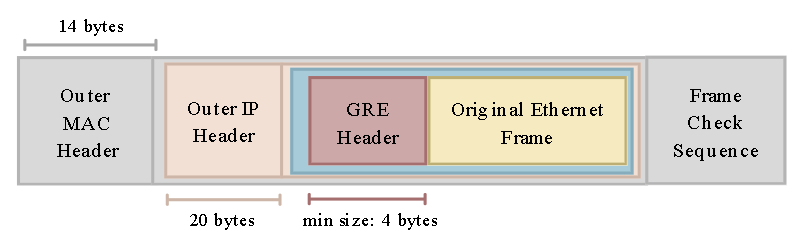
\includegraphics[width=0.6\linewidth]{Figures/NVGREpacket.png}
    \caption{NVGRE packet format. \cite{NVGRE}}
    \label{nvgre}
\end{figure}

The GRE header comprises the VSID field, which is 24 bits in length and enables the identification of up to approximately 16 million virtual networks. It also includes the FlowID field, which increases hash entropy for improved load distribution across equal-cost paths. Following this, the encapsulated tenant traffic, corresponding to the overlay network, includes the inner Ethernet header, containing the MAC addresses of the communicating virtual machines within the virtual network.

From a practical standpoint, this encapsulation process adds several bytes to the frame size. Consequently, the MTU of the underlay network must be increased to prevent fragmentation of the outer packets. Since NVGRE operates over an IP-based underlay, it benefits from Equal-Cost Multi-Path (ECMP) routing, enabling efficient distribution of flows across multiple available paths. The GRE Key field is one of the input parameters in the load-balancing hash calculation used for load balancing across these paths.

In terms of development, NVGRE has been primarily used in Microsoft-based environments, as it originated within Microsoft’s ecosystem and was standardized as the encapsulation method for Hyper-V Network Virtualization (HNV).

\subsection{Geneve}
Geneve is a network encapsulation protocol operating over UDP/IP, designed to provide extensibility through Type-Length-Value (TLV) options. Unlike VXLAN, Geneve decouples a minimal base header from an optional set of extension fields. The packet structure (Figure \ref{geneve}) is composed of outer Ethernet, IP and UDP headers, followed by the Geneve header and the encapsulated payload, which may include Ethernet and IP headers from the original frame.

\begin{figure} [H]
    \centering
    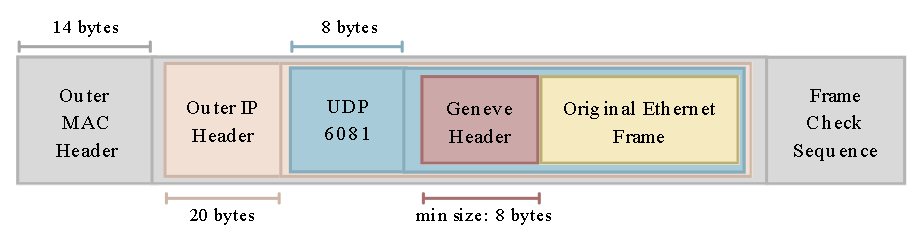
\includegraphics[width=0.65\linewidth]{Figures/genevePacket.png}
    \caption{Geneve packet structure. \cite{Geneve}}
    \label{geneve}
\end{figure}

Analysed from the outside in, we first encounter the Ethernet underlay header, which carriers frames between the GTEP, analogous to the VTEP in VXLAN, and the next hop. This header contains the source MAC of the GTEP and the destination MAC of the Layer 2 next hop. In the next layer, we encounter the IP underlay header, which transports the tunnel between the source and destination GTEPs, using their IP addresses.

Proceeding deeper into the encapsulation, we encounter the UDP header, which Geneve employs to introduce entropy for load balancing. The destination port assigned by IANA is 6081, while the source port is dynamically selected by the GTEP. The final header within the underlay is the Geneve, which is divided into an 8-byte base header and an optional block of Type-Length-Value (TLV) extensions. The base header is composed of several fields, most notably the VNI, which, as with other technologies, is the virtual network identifier. The optional TLV fields are used to attach supplementary information such as telemetry data or operational metadata.

After examining the outer encapsulation, attention shifts to the inner structure of the packet. Immediately following the Geneve header, the payload comprises the overlay frame, representing the original data frame generated by the VM. This frame includes its own set of link-layer, network-layer, and transport-layer headers, corresponding to the standard protocol stack within the virtualized environment.

Geneve is independent of the control plane, and to ensure proper distribution in ECMP, the endpoint varies the source UDP port to increase the entropy of the ECMP hash. Regarding security and Operations, Administration and Maintenance (OAM), the specification defines dedicated fields and behavioural guidelines, including the OAM bit and the handling of critical options, and recommends the use of IPsec when data integrity and confidentiality are required, as the encapsulation mechanism itself does not inherently provide these properties. 

In terms of support, Geneve has been widely adopted in software-based network infrastructures. The Linux kernel integrates a Geneve module that can be configured without relying Open vSwitch (OVS), while VMware NSX-T employs Geneve as its primary transport encapsulation protocol.

\subsection{Stateless Transport Tunnelling}

Stateless Transport Tunnelling (STT) is a comparatively recent addition to network virtualization technologies, developed as an alternative to existing protocols such as VXLAN and NVGRE. It is designed to support overlay networks within multi-tenant environments, providing tenants with control over their logical network domains. The primary objective of STT is to enhance the efficiency of network virtualization by encapsulating and forwarding packets between virtualized environments across a physical underlay network.

STT is one of the principal Layer 2 over Layer 3 tunnelling mechanisms used in network virtualization. Its distinguishing feature lies in the fact that STT packets are processed as standard TCP packets by physical Network Interface Cards (NICs). This allows NICs to leverage the TCP Segmentation Offload (TSO) capability to handle large STT packets efficiently. Under normal circumstances, large data payloads are divided at the TCP layer within the operating system kernel to maintain the size of each TCP segment below the Maximum Segment Size (MSS) threshold. With TSO, this segmentation process is offloaded to the physical NIC, thereby reducing CPU utilization on the host and improving overall performance.

In addition to TSO integration, STT exhibits several important characteristics. It employs MAC-in-IP tunnelling and uses 64-bit context identifiers, which significantly increase the number of possible virtual networks and enable broader service model scalability. The protocol achieves notable performance gains by exploiting hardware-based TSO capabilities, thereby minimizing the overhead associated with transmitting multiple small packets. STT operates in a stateless manner, with its packets supporting unicast communication between tunnel endpoints without relying on TCP windowing, synchronization or flow-control mechanisms. Moreover, STT can be implemented within software-based switches while still benefiting from hardware acceleration through compatible NICs, which substantially reduces the computational load on servers operating in high-bandwidth environments (10 Gbps and above).

Figure \ref{STT} shows the sequence of encapsulation and segmentation of a VM’s Ethernet frame at the transmitting endpoint. When the TSO feature is enabled on the virtual NIC, the virtual machine may generate large Ethernet frames. Then a tunnel endpoint, such as a virtual switch or a centralized virtual switch (CVSW), encapsulates the frame with STT and pseudo-TCP (P-TCP) headers. Finally, the underlying physical NIC subsequently divides the encapsulated frame into multiple smaller frames, each carrying consecutive sequence numbers within the P-TCP header. On the receiving side, the corresponding tunnel endpoint must reassemble the P-TCP segments prior to decapsulation, as only the first segment contains the STT and inner headers.

\begin{figure} [H]
    \centering
    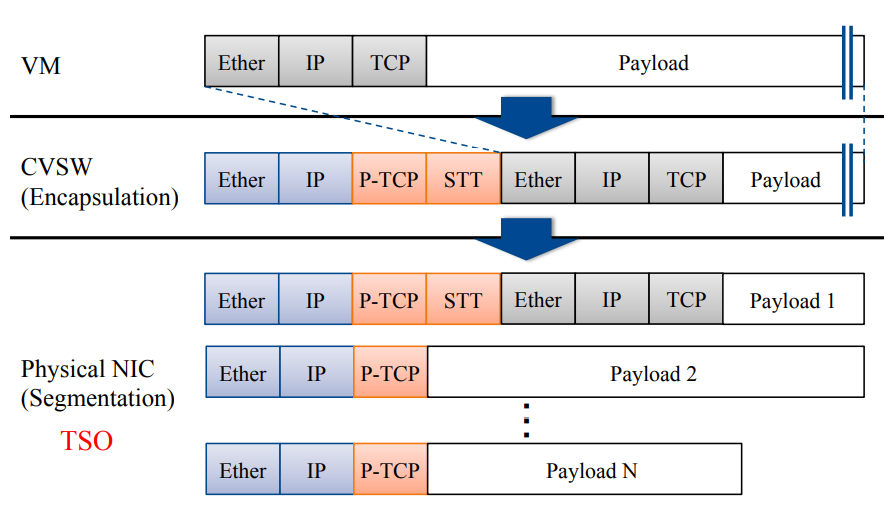
\includegraphics[width=0.55\linewidth]{Figures/STT.png}
    \caption{STT's encapsulation and segmentation flows with TSO feature. \cite{kawashima2020stt}}
    \label{STT}
\end{figure}

% ----------- 
\newpage

\nocite{*}
\printbibliography

\end{document}

